\documentclass{homework}
\usepackage[utf8]{inputenc}
\usepackage{amsmath}
\usepackage{amssymb}
\usepackage{braket}
\usepackage{graphicx}
\graphicspath{ {./images/} }

% CHANGE THE FOLLOW THREE LINES!
\newcommand{\hwname}{Sharath Chandra Sheripally}
\newcommand{\hwemail}{es18btech11016@iith.ac.in}
\newcommand{\hwnum}{1}

% CHANGE THESE ONLY ONCE PER CLASS
\newcommand{\hwtype}{Assignment}
\newcommand{\hwclass}{EE2101}

\begin{document}

\maketitle

\question*{Figure shows a quarter-car model commonly
used for analyzing suspension systems. The car's tire
is considered to act as a spring without damping, as
shown. The parameters of the model are \\

\begin{math}
M_b = car's body mass \\
M_{us} = wheel's mass \\
K_a = strut's spring constant \\
K_t = tire's spring constant \\
f_v = strut's damping constant \\
r = road disturbance (input) \\
x_s = car's vertical displacement \\
x_w = wheel's vertical displacement \\
\end{math}
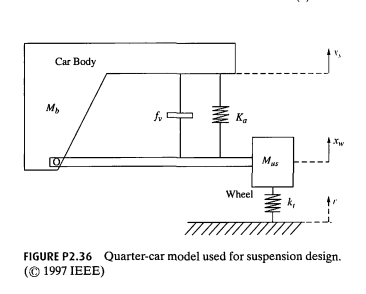
\includegraphics[scale=1]{figure1.png}}
 \\
\textbf{Soln.}
The two differential eqns for this system are \\
$M_b \ddot{x}_s + K_a(x_s - x_w) + C_a(\dot{x}_s - \dot{x}_w) = 0$ \\
$M_us \ddot{x}_w + K_a(x_w - x_s) + C_a(\dot{x}_w - \dot{x}_s) + K_t(x_w - r) = 0$
\\


Obtaining Laplace transform on both sides gives \\
$(M_b s^2 + C_a s + K_a) X_s - (K_a + C_a s) X_w = 0$ \\
$(M_{us} s^2 + C_a s + (K_a + K_t)) X_w - (K_a + C_a s) X_s = R K_t$
\\


Solving the first equation for $X_s$ and substituting into the second one gets \\
$\frac{X_w}{R} (s) = \frac{K_t (M_b s^2 + C_a s + K_a)}{(M_{us} s^2 + C_a s + (K_a + K_t)) (M_b s^2 + C_a s + K_a) - (K_a + C_a s)^2}$

\end{document}
